% ======================================================================
% Appendix (input after \appendix in paper.tex). No preamble.
% Sources: paper_ws/dossier_core.md (DC), paper_ws/dossier_posthoc.md (DP),
% research/fashion/RESULTS.md, research/fashion/output/paper_novelty/novelty_newcomer.csv,
% research/topics/output/hindsight_check.json, research/fashion/output/rq1_results.csv,
% research/fashion/output/posthoc/ph5_pivot/quintiles.csv, paper_ws/title_share.json.
% Tiers: A registered and replicated; B post hoc, supported by a declared held-out test;
% C registered, inconclusive or not replicated; D discovery only; E descriptive.
% ======================================================================

% ----------------------------------------------------------------------
\section{Data Provenance}\label{app:data}
% ----------------------------------------------------------------------

The herding account is tested on one complete submission population, so that neither the entry contrasts nor the
gate tests condition on acceptance. This appendix documents where the papers come from and which of them each test
uses.

\paragraph{Acquisition.} The corpus comes from our own dated acquisitions of official OpenReview records, reconciled
into 55,938 submission instances. Titles, abstracts, author-declared keywords, primary areas, author lists and
decisions all come from the selected official submission metadata; the keyword preprocessing is our own. The
discovery export holds 43,516 submissions and 219,719 declared author-list positions (positions, not distinct
people). The discovery corpus is the 43,480 submissions with a usable abstract of at least 30 words; 34 placeholders
and 2 malformed abstracts are dropped. Abstracts are a September 2026 snapshot, so accepted papers more often carry
camera-ready text: in 2023--2026, 17.6\% of accepted and 0.5\% of rejected abstracts contain a code link
(Appendix~\ref{app:gate} reports the link-removed re-run).

\paragraph{Splits.} Table~\ref{tab:app-years} gives papers by year. The held-out split is the 11,113 released
former-holdout papers, of which 11,099 have an abstract, released on 2026-10-18. They were this study's confirmation
split and had not been analysed before the held-out tests were registered. The source policy does not certify an
untouched, independent holdout. The source does not document how papers were assigned to the split, and it excluded
1,309 pending family or link cases. We therefore call the held-out tests a pre-registered out-of-sample replication, not a certified untouched
holdout. The two splits share conference-years, topic-year cells, reviewer pools and authors, so the held-out tests
guard against analyst overfitting but not against year- or reviewer-specific patterns. The pooled corpus (54,579
papers) is used only for the exploratory re-run (Appendix~\ref{app:tests}).

\begin{table}[t]
\centering\footnotesize
\begin{tabular}{@{}lrr@{}}
\toprule
Year & Discovery & Held-out \\
\midrule
2017 & 384 & 105 \\
2018 & 770 & 212 \\
2019 & 1,248 & 309 \\
2020 & 2,070 & 500 \\
2021 & 2,360 & 603 \\
2022 & 2,649 & 704 \\
2023 & 3,872 & 995 \\
2024 & 5,765 & 1,445 \\
2025 & 8,951 & 2,284 \\
2026 & 15,411 & 3,942 \\
\midrule
All & 43,480 & 11,099 \\
\bottomrule
\end{tabular}
\caption{Papers with a usable abstract by year. Discovery: 2017--2020 4,472; 2021--2023 8,881; 2024--2026 30,127
(69.3\%). Submissions grew 40.1-fold from 2017 to 2026. Outcome-free.}
\label{tab:app-years}
\end{table}

\paragraph{Analysis populations.} Field analyses use all discovery papers (the registered field tests: 43,096 papers
from 2018--2026; H1d and H1e 42,990). Entry analyses use the 42,325 papers from 2019--2026 with at least one author
identifier (42,315 in 776 topic-year cells after singleton cells are dropped). Acceptance tests use the 32,190
ordinary submissions from 2018--2026 with a final accept or reject decision (40.1\% accepted); the 9,986 withdrawn
submissions are left out. Held-out populations are 10,978 papers (H1d), 10,718 (entry) and 8,185 decided papers from
2018--2026 (acceptance; 8,284 decided in all). The post hoc gate modules use decided 2023--2026 papers
(Appendix~\ref{app:gate}).

\paragraph{Existing collections, audited and not pooled.} Re$^2$ \citep{zhang2025re2} was initially considered as the
main dataset and audited: its main-conference ICLR coverage ends in 2023 and omits 2019, its conversations contain
training-format placeholders, and its rebuttal train and test partitions share 475 paper identifiers. The audit
motivated our own collection. A public GitHub archive of ICLR rebuttal records (\texttt{iclr-rebuttal-analysis})\footnote{\url{https://github.com/MlouisBE/iclr-rebuttal-analysis}}
served as a separate layer for source comparison and identity reconciliation; it added no submissions and supplies no
text. A public metadata archive (Paper Copilot)\footnote{Described in arXiv:2510.13201.} was used for metadata comparisons and documents the lineage of reconstructed
2024--2025 review-score pairs; this study uses no review scores. None of the three is pooled into the analytical
corpus.

\paragraph{What this means for the test.} Because rejected and withdrawn submissions are present, what topic
newcomers write is observed for every paper they submitted, and the gate tests compare accepted with rejected papers
of the same topic and year. Neither half of the herding account is tested on survivors only.

% ----------------------------------------------------------------------
\section{Measurement Validation}\label{app:measure}
% ----------------------------------------------------------------------

Each prediction that separates imitation from continuity is measured with four instruments: topics, contribution
labels, entry status, and distances in one embedding space. This appendix reports how far each can be trusted.

\paragraph{Topics.} Title and abstract (``title [SEP] abstract'') are embedded with SPECTER2
\citep{cohan2020specter,singh2023scirepeval} (base model with the proximity adapter), reduced by unit-length PCA to
128 dimensions (93\% of the variance), and clustered by spherical $k$-means with $k=100$ (best of 3 seeds $\times$ 20
initialisations). A broad level (20 topics, Ward) and a fine level (198 topics) are supplementary. The topic layer
reads no acceptance, decision or review field; an output validator checks this. Topics hold 127--1,121 papers; 91
topics (94\% of papers) have at least 30 papers in at least three years. On 2024--2026 papers, normalised mutual
information (NMI) with ICLR's primary areas is 0.302, against 0.272 for a TF-IDF/LSA word-count baseline, and
synonym overlap is 0.67 against 0.46. In a blind name check, the correct topic was picked for 80\% of items at this
level and for 61\% at the fine level (chance 10\%). The adjusted Rand index (ARI) across seeds is 0.66 (0.63--0.69);
the median Jaccard overlap is 0.66, with 26 topics below 0.5. Table~\ref{tab:app-k} gives the sensitivity to $k$:
$k=100$ was fixed before the sweep (a design choice, not tuned), and adjacent solutions nest only partly (76--82\% of a
finer topic's papers fall in one coarser topic). Table~\ref{tab:app-ktests} shows that the registered estimates keep
their sign at $k=75$ and $k=150$, except the inconclusive H2a at $k=150$.

\begin{table}[t]
\centering\footnotesize
\setlength{\tabcolsep}{3.5pt}
\begin{tabular}{@{}rrrrrrr@{}}
\toprule
$k$ & Track. & NMI & ARI & Syn. & Coh. & NMI$_{100}$ \\
\midrule
50 & 100\% & 0.294 & 0.77 & 0.77 & 0.26 & 0.72 \\
75 & 97\% & 0.302 & 0.74 & 0.72 & 0.27 & 0.80 \\
\textbf{100} & \textbf{94\%} & \textbf{0.302} & \textbf{0.68} & \textbf{0.67} & \textbf{0.29} & 1 \\
150 & 76\% & 0.301 & 0.62 & 0.67 & 0.31 & 0.78 \\
200 & 53\% & 0.302 & 0.57 & 0.64 & 0.33 & 0.75 \\
\bottomrule
\end{tabular}
\caption{Topic quality by $k$ (sensitivity sweep). Track.: papers in trackable topics; NMI with ICLR primary areas;
ARI across seeds in the sweep (the main map's own seed ARI is 0.66); Syn.: synonym overlap; Coh.: keyword coherence;
NMI$_{100}$: NMI with the $k=100$ map. Outcome-free (E).}
\label{tab:app-k}
\end{table}

\begin{table}[t]
\centering\footnotesize
\setlength{\tabcolsep}{4pt}
\begin{tabular}{@{}lrrr@{}}
\toprule
Test (unit) & $k=75$ & $k=100$ & $k=150$ \\
\midrule
H1d (pp, 0$\to$100\% FM) & $-$8.70 & $-$7.98 & $-$7.47 \\
H2b (pp) & +3.06 & +3.71 & +3.87 \\
H2c (pp) & $-$1.51 & $-$1.70 & $-$1.81 \\
H2a (pp) & $-$1.39 & $-$0.73 & +0.37 \\
H3a (pp per log unit) & $-$1.54 & $-$1.68 & $-$1.33 \\
\bottomrule
\end{tabular}
\caption{Registered discovery estimates at three values of $k$ (counted variants). Intervals for $k=100$ are in
Table~\ref{tab:app-tests}. H3a is inconclusive at every $k$.}
\label{tab:app-ktests}
\end{table}

\paragraph{Contribution labels.} Each paper receives one primary contribution type from a fixed LLM codebook (prompt
v1): method (including new architectures, type ``model''), theory, empirical, dataset/benchmark, evaluation, other.
A measurement paper is a dataset/benchmark or evaluation paper. An FM paper uses or adapts a large pre-trained model
(an LLM, CLIP or a pre-trained diffusion model), coded with the same codebook. Labels were produced by Claude Haiku
subagents with the prompt unchanged, in batches of 100; this replaced a planned external run and is a logged
deviation. The registered quality gate required at least 93\% agreement with a 300-paper pilot and a second-pass
$\kappa \geq 0.80$; the run achieved 97.7\% and $\kappa$ 0.93. Against a reference set of 2,300 papers labelled by
LLM annotators, main-class agreement is 95.8\% (pilot 300: 97.7\%; 200 double-labelled training papers: 95.5\%;
1,800 single-labelled: 95.6\%). A blind second pass on 2,174 discovery papers gives $\kappa$ 0.93 overall, 0.933 for
method (97.5\% agreement) and 0.949 for measurement (99.3\%). Relative to the LLM reference on its random stratum,
false-positive and false-negative rates are 0.084 and 0.011 for method, and 0.005 and 0.070 for measurement; the S8
variant rescales the entry estimates by them, which can only enlarge them (+4.09 and $-$1.84\,pp). On 555 held-out
papers, agreement is 96.9\% for the main class ($\kappa$ 0.931), 98.0\% for method (0.949), 99.1\% for measurement
(0.923) and 98.2\% for FM (0.960). These figures show consistency between LLM labellings more than human-level
validity. Over all discovery papers, the class mix is method 75.1\%, empirical 6.9\%, theory 6.9\%, dataset/benchmark
5.2\%, other 3.5\% and evaluation 2.4\%; the measurement share rose from 2.6\% (2017) to 11.1\% (2026) (E).

\paragraph{Keywords.} Author keywords are canonicalised to 40,930 expressions. The 912 keywords with at least 20
papers were typed by two LLM annotators ($\kappa$ 0.93; 96.6\% agreement; 31 adjudicated). Keyword states use a
759-keyword vocabulary. Held-out papers carry raw keywords only; a lookup learned on discovery papers alone maps
45,778 forms (5,738 of them non-identity), with cross-validated recall and precision of 98.6\% and 99.96\% on the
759-keyword vocabulary, 99.0\% and 99.98\% on the 68 frequent keywords, and 97.2\% and 100\% for ``federated
learning''.

\paragraph{Entry status.} A paper is an incumbent paper if at least one author identifier has an earlier ICLR
submission, with any outcome, in the paper's topic, strictly before the paper's year; otherwise it is a newcomer
paper. Exact identifiers are used, never names. ICLR author identifiers were 98--99.6\% e-mail-based in 2017--2020,
85\% profile-based in 2021 and fully profile-based in 2025--2026, and the two kinds are not linked. Earlier histories
are therefore hidden after 2020: incumbency on the all-years map falls from 18\% (2020) to 0.5\% (2021) and recovers
to 18\% (2022) and 33\% (2026). This turns some true incumbents into newcomers and pulls entry contrasts towards zero.
The counted R2 variant drops only 2021--2022 and leaves the entry results unchanged: +3.72 [+2.61, +4.83] and $-$1.74
[$-$2.53, $-$0.95] pp ($n$ 37,312). Earlier work that sits in the held-out split is invisible to discovery histories,
which also pulls towards zero. Held-out features were built on pooled histories (held-out incumbency 30.9\%).
Discovery incumbency is 26.5\% under discovery-only histories; under pooled histories it would be 30.0\%, with 1,515
discovery papers switching from newcomer to incumbent. Experience at other venues is not captured.

\paragraph{Probable earlier versions.} 170 discovery papers are flagged as probable resubmissions: 167 have an earlier
paper at centred SPECTER2 cosine $\geq \tau = 0.90$, and 3 an earlier paper with an identical normalised title. The
threshold was calibrated by blind LLM judges (two Haiku runs and one Sonnet run), whose yes-rates were 10\%, 48\%,
90\% and 100\% across four cosine bins. The flags define the R1 and S4 variants and the exclusions in both distance
measures.

\paragraph{Distances.} Both distances use SPECTER2 vectors centred with a frozen discovery mean and L2-normalised.
Closeness to the team's own record ($F_{\max}$) is, for each experienced author, the cosine between the paper's vector
and the normalised mean of that author's earlier ICLR submissions since 2021, excluding the paper's probable earlier
version and any paper at cosine $\geq 0.90$; $F_{\max}$ is the maximum over experienced authors. The measure follows
\citet{bao2025persistence}. Distance from earlier ICLR work is $1-$ the mean cosine to the 10 nearest submissions
from strictly earlier years, as a percentile within topic $\times$ year (Appendix~\ref{app:distance}). The space is
the same; the reference points differ.

\paragraph{A dropped measure.} A registered measure of buzzword use (a fast-growing keyword used atypically) failed
its blind validation: LLM judges rated 42\% (95\% CI 33--52\%) of flagged uses peripheral, against 15\% of matched
non-flagged uses, and the registered gate required at least 50\%. Its two hypotheses (H2d, H3c) were dropped before
any estimate; exploratory rows that use it are reported and not interpreted.

\paragraph{Held-out topic maps.} For each of nine alternative maps ($k=50$, 75, 150 and 200, the seed refit, the
year-balanced map and the maps fitted on 2017--2020, 2021--2023 and 2024--2026), the exact centres were re-derived
from the frozen fits; every re-derivation reproduces all saved discovery labels. On every map the held-out topic
distribution differs from discovery by no more than sampling noise, and the share of stable papers is 0.792 in both
splits.

\paragraph{What this means for the test.} The labels are consistent rather than validated against human judgement,
and the identifier switch hides earlier histories. The switch pulls the entry contrasts towards zero, as does label
error if it is non-differential, so neither can produce the reversal of the registered herding prediction.

% ----------------------------------------------------------------------
\section{Hindsight Details}\label{app:hindsight}
% ----------------------------------------------------------------------

The herding reading starts from vivid waves. Section~\ref{sec:field} shows that the number of emerging topics a map finds depends on
the years used to fit it. This appendix gives the six maps in full and three further results that depend on the
fitting years.

\paragraph{Six maps on the same papers.} All maps use $k=100$, the same 43,480 papers and the same pipeline; only the
fitting years differ (Table~\ref{tab:app-maps}). A topic is emerging if its 2024--2026 share is at least three times
its 2017--2020 share, and declining if it is at most a third. Because 69\% of papers are from 2024--2026, the
all-years map is in effect a present-day map: it fits 2026 papers better than 2017 papers (mean similarity to the
assigned centroid 0.65 against 0.62), while the 2017--2020 map does the reverse (0.69 against 0.53). Growth compounds
hindsight: the all-years map finds as many emerging topics as the map fitted on 2024--2026 alone (29 against 28). The
share of 2024--2026 papers in emerging topics brackets the effect, from 22.3\% on the 2017--2020 map to 40.9\% on the
all-years map (20.9--42.2\% across the six maps), rather than pinning it down: the early map cannot represent topics born after 2020, and the maps differ in fitting corpus as well as in
window (E).

\begin{table}[t]
\centering\footnotesize
\setlength{\tabcolsep}{3pt}
\begin{tabular}{@{}lrrrc@{}}
\toprule
Map (fitted on) & ARI & Emerging & Declining & Fit 2017/26 \\
\midrule
All years & 1 & 29 (40.9) & 13 (41.7) & 0.62/0.65 \\
Seed refit & 0.69 & 28 (40.9) & 15 (43.2) & 0.62/0.65 \\
Year-balanced & 0.48 & 16 (42.2) & 26 (38.6) & 0.69/0.61 \\
2024--2026 & 0.55 & 28 (31.0) & 6 (30.2) & 0.56/0.66 \\
2021--2023 & 0.40 & 10 (20.9) & 17 (31.6) & 0.63/0.58 \\
2017--2020 & 0.34 & 8 (22.3) & 17 (21.9) & 0.69/0.53 \\
\bottomrule
\end{tabular}
\caption{Six $k=100$ maps that differ only in their fitting years. ARI with the all-years map. Emerging: count
(share of 2024--2026 papers in them, \%). Declining: count (share of 2017--2020 papers in them, \%). Fit: mean
similarity of a year's papers to their assigned centroid. Outcome-free (E).}
\label{tab:app-maps}
\end{table}

\paragraph{Diversity is not a finding.} The effective number of topics per year (as a share of $k$) peaks inside
each map's own fitting years (Table~\ref{tab:app-div}): in 2020 on the 2017--2020 map, in 2022 on the 2021--2023 map,
in 2025 on the 2024--2026 and all-years maps, and in 2021 on the year-balanced map. The all-years map's rise in
diversity to 2025 is therefore a property of where the map was fitted, not a finding about the field.

\begin{table}[t]
\centering\footnotesize
\setlength{\tabcolsep}{3.5pt}
\begin{tabular}{@{}lrrrrrr@{}}
\toprule
Year & All & Seed & Bal. & 24--26 & 21--23 & 17--20 \\
\midrule
2017 & 0.443 & 0.470 & 0.636 & 0.448 & 0.556 & 0.738 \\
2018 & 0.525 & 0.529 & 0.743 & 0.496 & 0.655 & 0.850 \\
2019 & 0.582 & 0.589 & 0.808 & 0.520 & 0.745 & 0.888 \\
2020 & 0.660 & 0.665 & 0.850 & 0.574 & 0.833 & \textbf{0.908} \\
2021 & 0.703 & 0.713 & \textbf{0.867} & 0.619 & 0.915 & 0.867 \\
2022 & 0.725 & 0.731 & 0.831 & 0.629 & \textbf{0.921} & 0.804 \\
2023 & 0.797 & 0.795 & 0.847 & 0.697 & 0.911 & 0.785 \\
2024 & 0.897 & 0.893 & 0.820 & 0.842 & 0.839 & 0.792 \\
2025 & \textbf{0.910} & \textbf{0.896} & 0.731 & \textbf{0.937} & 0.739 & 0.731 \\
2026 & 0.840 & 0.831 & 0.634 & 0.930 & 0.640 & 0.681 \\
\bottomrule
\end{tabular}
\caption{Effective number of topics divided by $k$, by year and map (maximum in bold). Each map is most diverse in
its own fitting years. Outcome-free (E); not a finding.}
\label{tab:app-div}
\end{table}

\paragraph{Topic growth looks predictable only in hindsight.} An out-of-time forecast of two-year topic growth (test
origins 2021--2024; post hoc, outcome-free) shows the same asymmetry (Table~\ref{tab:app-forecast}). On the all-years
map, small topics grow: topic size ``predicts'' growth with $R^2$ 0.28. On the 2017--2020 map it does not ($R^2$
$-$0.03). The in-sample chance of top-fifth growth by size tercile is 40\%, 21\% and 2\% (small, middle, large) on
the all-years map, against 22\%, 20\% and 20\% on the early map. Caveats: the early map cannot represent topics born
after 2020, the maps differ in fitting corpus and eligibility timing, so the gap cannot be attributed to hindsight
alone, and there is no paired test. Genuine forecasting is weak: on the early map, momentum's top-fifth picks are right for
only 16 of 56 (29\%) for origins 2021--2023.

\begin{table}[t]
\centering\footnotesize
\setlength{\tabcolsep}{3.5pt}
\begin{tabular}{@{}lrr@{}}
\toprule
Predictor: metric & All years & 2017--2020 \\
\midrule
Size: $R^2$ & 0.281 & $-$0.033 \\
Size: Spearman & 0.595 & $-$0.043 \\
Size: precision, top fifth & 0.563 & 0.250 \\
Size: $R^2$ without LLM/VLM areas & 0.30 & $-$0.09 \\
Momentum: $R^2$ & 0.056 & 0.032 \\
Momentum: Spearman & 0.377 & 0.198 \\
Momentum: precision, top fifth & 0.420 & 0.395 \\
Topic-years & 446 & 522 \\
\bottomrule
\end{tabular}
\caption{Out-of-time forecasts of two-year topic growth, test origins 2021--2024. Intervals for size: $R^2$ [0.217,
0.335] against [$-$0.082, $-$0.002]; Spearman [0.510, 0.672] against [$-$0.151, 0.063]. Chance precision is 0.20.
Post hoc, outcome-free (E).}
\label{tab:app-forecast}
\end{table}

\paragraph{The lifecycle answer depends on the map.} The registered tests of whether topics ``age'' from method to
measurement work (H1a--c) show nothing on the all-years map: method $-$0.14 [$-$1.78, +1.49] and measurement +0.50
[$-$0.76, +1.75] pp per log unit of prior papers (C). On the 2017--2020 map applied to 2021--2026 papers, the method
and measurement estimates point the predicted way: $-$3.48 [$-$6.21, $-$0.76] and +3.96 [+1.35, +6.57] (counted
variants, read as a lifecycle only in exploratory and unadjusted terms). The empirical share (H1c) has the wrong sign
on every map. Table~\ref{tab:app-life} lists every counted variant. By the registered rule all three are not
supported, because the main map shows nothing; the lesson is that the answer depends on the map.

\begin{table}[t]
\centering\footnotesize
\setlength{\tabcolsep}{2pt}
\begin{tabular}{@{}lrrrr@{}}
\toprule
Variant & H1a ($-$) & H1b (+) & H1c (+) & $n$ \\
\midrule
All-years (main) & $-$0.14 & +0.50 & $-$0.31 & 43,096 \\
$k=75$ & $-$0.10 & +0.93 & $-$0.74 & 43,096 \\
$k=150$ & $-$0.35 & +0.69 & $-$0.13 & 43,096 \\
Year-balanced$^h$ & $-$0.08 & +0.66 & $-$0.75 & 43,096 \\
Early map, all papers & $-$2.30 & +2.16 & $-$1.06 & 43,096 \\
Early map, 2021--2026$^h$ & $-$3.48 & +3.96 & $-$1.03 & 39,008 \\
Stable papers & +0.53 & +0.28 & $-$0.37 & 34,144 \\
Coherent topics & $-$0.20 & +0.50 & $-$0.26 & 42,161 \\
Certain labels & $-$0.66 & +0.92 & $-$0.56 & 26,369 \\
Without 2026 & +0.48 & $-$0.53 & $-$0.16 & 27,685 \\
\bottomrule
\end{tabular}
\caption{Topic crowding and contribution mix: every counted variant of the registered H1a (method share), H1b
(measurement share) and H1c (empirical share), pp per log unit of prior topic papers; registered sign in
parentheses; $^h$ hindsight variant; early map: fitted on 2017--2020. Predicted sign: 7/9, 8/9 and 0/9 variants. Outcome-free labels.}
\label{tab:app-life}
\end{table}

\paragraph{What this means for the test.} A herd reading starts from the waves, and the emergence a field history shows
is partly a property of when its map was fitted. For this reason every registered time-trend claim had to hold on
the year-balanced map and on the 2017--2020 map applied to 2021--2026 papers. H1d, the package result, passes both;
the lifecycle claims do not.

% ----------------------------------------------------------------------
\section{Every Registered and Declared Test}\label{app:tests}
% ----------------------------------------------------------------------

The negative half of our thesis rests on registered tests and the positive half on post hoc tests with declared
held-out tests. This appendix lists every such test, including those that failed, so that the denominators are
visible (Table~\ref{tab:app-tests}).

\paragraph{Protocol.} Hypotheses, models, the support rule and the robustness variants were registered on 2026-10-13,
before any full-corpus label existed (only the 2,300 validation papers had labels, and no hypothesis had been tested
on them). Earlier exploratory work on keyword popularity and title style in the same corpus came before registration
and is disclosed. A hypothesis is \emph{supported} only if its main estimate has the predicted sign, its Holm-adjusted
$p$ is below 0.05 within its family \citep{holm1979simple}, at least 75\% of its counted variants have the predicted
sign, and both hindsight variants (year-balanced map; 2017--2020 map on 2021--2026 papers) have the predicted sign.
Otherwise the verdict is ``significant in the opposite direction'' (Holm $p<0.05$ with the wrong sign), ``equivalent
to null'' (90\% CI inside the smallest effect of interest) or ``inconclusive''. Discovery Holm families were
\{H1a--e\}, \{H2a--c\} and \{H3a--b\}. Linear probability models use topic and year (or topic $\times$ year) fixed
effects with standard errors clustered by topic (100 clusters). Outcomes were readable only through a sealed loader,
which ran once inside the frozen run (18 seconds). Nine adversarial review rounds preceded the freeze; two blinding
incidents are disclosed (a reviewer saw one exploratory estimate on the failed buzzword measure, and the analyst once
read the value sets of outcome columns).

\paragraph{Held-out tests.} Held-out tests were registered on 2026-10-18 and run once (16:39--16:42 UTC). Every test
is one-sided at $\alpha = 0.05$: $p_1 = p/2$ if the estimate has the predicted sign, otherwise $1-p/2$, where $p$ is
the two-sided $p$ of the discovery method; the exception is premia $b$, whose $p_1$ is the intersection-union $p$
for $0<b<1$ (0.003). Holm families were \{H1d\}, \{H2b$'$, H2c$'$\}, \{H3a\}, \{H4-FL\} and the
post hoc primary pair \{E1, P1b\}. Six post hoc secondary tests (E4, P7, teams H1, A1, premia $b$, premia D0) are each
one-sided at 0.05 and unadjusted, so one false positive among them would not be surprising; their Holm values hold
within their own module only (teams H1 about 0.17 across modules, A1 about 0.18). The PH6 wave test was declared on
2026-10-28 and run once. H2b$'$ and H2c$'$ reverse the registered herding predictions, which failed in discovery;
they were registered after discovery and before any held-out data existed.

\begin{table*}[p]
\centering\footnotesize
\setlength{\tabcolsep}{3pt}
\begin{tabularx}{\textwidth}{@{}>{\raggedright\arraybackslash}X l l l l >{\raggedright\arraybackslash}p{2.45cm}@{}}
\toprule
Test (predicted sign; held-out $n$) & Discovery [95\% CI] & Held-out [95\% CI] & $p_1$ & MDE80 & Verdict (tier) \\
\midrule
\multicolumn{6}{@{}l}{\textit{Field: registered 2026-10-13; H1d also registered for held-out papers}} \\
H1a method share $\sim$ crowding ($-$) & $-$0.14 [$-$1.78, +1.49] & not tested & & & not supported (C) \\
H1b measurement share $\sim$ crowding (+) & +0.50 [$-$0.76, +1.75] & not tested & & & not supported (C) \\
H1c empirical share $\sim$ crowding (+) & $-$0.31 [$-$1.29, +0.67] & not tested & & & not supported (C) \\
H1d new-architecture share $\sim$ prior FM adoption, 0$\to$100\% ($-$; 10,978) & $-$7.98 [$-$12.14, $-$3.82] & $-$11.0 [$-$18.1, $-$3.9] & 0.0013 & 12.0 & supported (A) \\
H1e empirical or evaluation share $\sim$ prior FM adoption (+) & $-$0.63 [$-$3.64, +2.38] & not tested & & & not supported (C) \\
\midrule
\multicolumn{6}{@{}l}{\textit{Entry: registered 2026-10-13; reversed H2b$'$ and H2c$'$ registered for held-out papers after discovery}} \\
H2a incumbent share $\sim$ hot topic ($-$) & $-$0.73 [$-$2.68, +1.22] & not registered$^u$ & & 3.6$^f$ & inconclusive (C) \\
H2b method paper $\sim$ newcomer paper ($-$); reversed H2b$'$ (+; 10,718) & +3.71 [+2.61, +4.80] & +3.60 [+1.48, +5.71] & 0.0007 & 2.8 (1.7$^f$) & failed; reversal supported (A) \\
H2c measurement paper $\sim$ newcomer paper (+); reversed H2c$'$ ($-$; 10,718) & $-$1.70 [$-$2.46, $-$0.93] & $-$2.10 [$-$3.35, $-$0.85] & 0.0005 & 2.4 (1.1$^f$) & failed; reversal supported (A) \\
\midrule
\multicolumn{6}{@{}l}{\textit{Gate: registered 2026-10-13 (H3a also for held-out papers); H4-FL registered 2026-10-17, before any held-out data}} \\
H3a acceptance $\sim$ crowding, per log unit ($-$; 8,185) & $-$1.68 [$-$3.68, +0.32] & $-$1.51 [$-$5.20, +2.19] & 0.21 & 4.8 & inconclusive; uninformative (C) \\
H3b acceptance $\sim$ crowding $\times$ method paper ($-$) & $-$0.36 [$-$1.51, +0.79] & not registered$^u$ & & 2.4$^f$ & inconclusive (C) \\
H4-FL federated-learning keyword, level ($-$; 134 FL papers) & $-$11.3 [$-$17.9, $-$4.8] & $-$4.9 [$-$15.4, +5.7] & 0.14 & 14.5 & not supported; uninformative (C; discovery D) \\
H4-FL trend, pp per year ($-$) & $-$3.0 [$-$6.4, +0.5] & +3.2 [$-$3.3, +9.6] & 0.88 & n.c. & not supported, opposite sign (C) \\
\midrule
\multicolumn{6}{@{}l}{\textit{Gate: post hoc in discovery (declared before run); held-out tests declared 2026-10-18 (PH6: 2026-10-28)}} \\
E1 far jump: $F_{\max}$ p10 $-$ p50 ($-$; 5,344) & $-$5.44 [$-$7.10, $-$3.78] & $-$6.09 [$-$9.32, $-$2.86] & 0.0025 & 4.9 (0.89) & supported, primary (B) \\
P1b field distance: least-distant fifth $-$ middle fifth ($-$; 8,010) & $-$3.27 [$-$4.93, $-$1.60] & $-$0.13 [$-$3.50, +3.25] & 0.47 & 5.4 (0.47) & not supported; uninformative (C; discovery D) \\
E4 within-author closeness, per +0.1 cosine (+; 4,311) & +0.55 [+0.21, +0.90] & +1.06 [+0.23, +1.89] & 0.006 & n.c. & supported, secondary (B) \\
P7 within-author field distance, per 10 percentile points (+; 4,810) & +0.39 [+0.09, +0.69] & +0.34 [$-$0.47, +1.16] & 0.22 & $\approx$1.0--1.1$^d$ & not supported (C) \\
Teams H1: one topic insider vs none (+; 6,243) & +3.42 [+1.18, +5.66] & +3.88 [+0.28, +7.47] & 0.017 & $\approx$4.5$^d$ & supported, secondary (B) \\
A1 Emerging $-$ Mainstream keyword (+; 5,741) & +2.67 [+0.76, +4.58] & +3.25 [$-$0.18, +6.69] & 0.031$^n$ & $\approx$4.3$^d$ & supported, weak: CI includes 0 (B weak) \\
Premia $b$: 2024--2026 topic edge on 2018--2022 edge ($0<b<1$; 75 units) & 0.38 [0.18, 0.58] & 0.60 [0.32, 0.88] & 0.003$^i$ & n.c. & supported, secondary (B) \\
Premia D0: EB-shrunk edges predict better than zero, $\times10^{-3}$ (+) & none (new test) & 1.71 [0.42, 3.01] & 0.005 & n.c. & supported, secondary (B) \\
PH6 waves: gap after $-$ up to a keyword's share peak ($-$; 17 waves) & $-$5.7 [$-$8.5, $-$2.9]$^t$ & $-$5.2 [$-$11.1, +0.7] & 0.043 & 7.4 & supported, only just: CI includes 0 (B weak) \\
\bottomrule
\end{tabularx}
\caption{Every registered and declared test. Estimates in pp within topic and year (H1d: change in the
new-architecture share for prior-year FM adoption from 0 to 100\%; keyword and wave rows: against all other papers of
the same year). Discovery intervals $\pm$1.96 SE; the held-out H1d interval uses $t(G-1)$ quantiles. $p_1$: held-out
one-sided $p$; Holm-adjusted, it is unchanged except for H2b$'$ and H2c$'$ (0.0010 each) and E1 (0.0050). MDE80:
held-out minimum detectable effect at 80\% power, registered unless marked, with power at the discovery effect for E1
and P1b in parentheses; $^f$ discovery MDE80 from the frozen dry run; $^d$ derived post hoc ($2.49\times$SE), with
no reading rule; n.c.\ not computed. $^u$ unregistered held-out row (Table~\ref{tab:app-unreg}). $^n$ null-frame
$p_1$ 0.020; two-sided $p$~0.063. $^i$ intersection-union $p$ for $0<b<1$. $^t$ not a test. Tiers as in Table~\ref{tab:main};
reading rules in the text.}
\label{tab:app-tests}
\end{table*}

\begin{figure}[t]
  \centering
  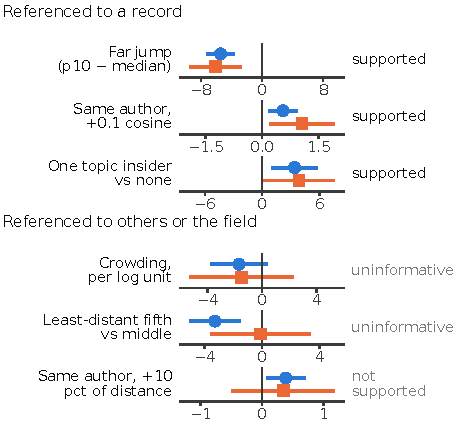
\includegraphics[width=\columnwidth]{figs/fig4b_tests.pdf}
  \caption{Gate tests by reference point: discovery (blue circles),
  held-out (orange squares), 95\% intervals, each row on its own axis, held-out verdict at right. `Others or the
  field' groups crowding (others now) with distance from earlier ICLR work (the field's record); `Same author, +10 pct
  of distance' is the within-author slope for that distance. Compare replication status, not size. All rows except
  crowding (registered H3a) were post hoc in discovery; held-out tests are one-sided, and the same-author and insider
  tests are secondary and unadjusted.}
  \label{fig:gate-tests}
\end{figure}

\paragraph{Discovery details.} H1a--c, H1e: Holm 1.0; predicted sign in 7/9, 8/9, 0/9 and 4/9 counted variants
(H1c also fails both hindsight variants). H1d: Holm 0.0014; 9/9 variants ($-$6.3 to $-$14.2). H2a: Holm 0.46; 8/10
variants with the predicted sign, but the year-balanced hindsight variant has the wrong sign (+1.05), as does $k=150$
(+0.37); the two early-map variants are $-$1.62 ($p$~0.03) and $-$1.55 ($p$~0.045); TOST $p$~0.10. H2b and H2c: wild
cluster restricted bootstrap $p < 1/9{,}999$, Holm $<0.001$ with the wrong sign; all 10 counted variants share the
observed sign (+2.16 to +3.87; $-$1.81 to $-$0.86), as do both hindsight variants (+3.10 and +2.16; $-$1.41 and
$-$0.86). With log team size, H2c shrinks to $-$0.54 [$-$1.11, +0.04] ($p$~0.07) while H2b stays at +3.92; by era,
H2c is concentrated in 2024--2026 ($-$2.0, against $-$0.5 n.s.\ in each earlier era). H3a: Holm 0.20; all 11
counted variants negative ($-$2.53 to $-$1.31; logit average marginal effect $-$1.64); supplementary variants are
negative and some nominally significant (team size $-$2.04, fine topics $-$2.42, withdrawals after review counted as
rejections $-$2.12, newcomer control $-$2.99), but they are unadjusted and outside the verdict; TOST $p$~0.75. H3b:
Holm 0.53; 10/11 variants negative; TOST $p$~0.14. No non-supported hypothesis is equivalent to null.

\paragraph{Held-out details.} H1d: 9/9 variants negative ($-$5.4 to $-$15.2); the weakest, the prospective early-map
variant, is $-$5.4 (two-sided $p$~0.24). H2b$'$ and H2c$'$: 10/10 variants, both hindsight variants pass; two-way
clustering agrees (Holm $p_1$ 0.0010 and 0.0009); the stress sensitivity gives Holm $p_1$ 0.0075 for both; no variant
is significant against the prediction. With log team size, H2c$'$ shrinks to $-$0.98 (two-sided $p$~0.10) while
H2b$'$ stays at +3.64, as in discovery. H3a: 9/11 variants negative; the hindsight requirement fails (early map on
2021--2026 papers +1.44); TOST $p$~0.61. H4-FL: yearly held-out gaps of $-$20.0, $-$16.9, +6.4, $-$3.6, $-$11.3 and
$-$0.2\,pp (2021--2026, on 13--36 papers a year); the discovery pattern of about $-$11 to $-$15\,pp in every year since
2023 does not appear.

\paragraph{Reading rules.} Four supported tests were underpowered at the discovery effect: H1d (MDE80 12.0 against
$-$7.98), H2c$'$ (2.4 against $-$1.70), teams H1 ($\approx$4.5 against +3.42) and A1 ($\approx$4.3 against +2.67).
They confirm direction, not size; among underpowered tests, the significant ones tend to overstate the effect. A
non-supported registered test whose estimate is below its MDE80 (H3a, H4-FL, P1b) is uninformative, not evidence of no
association. A1's 95\% interval includes 0 because a one-sided 5\% test corresponds to a 90\% interval.

\paragraph{Further notes to Table~\ref{tab:main}.} Row 6 (distance from earlier ICLR work): outcome-free,
unregistered and added during writing; among method papers the gap is +5.24 [+4.16, +6.31]; ``own work excluded''
means that every earlier paper sharing an author with the paper is removed from its reference set
(Appendix~\ref{app:distance}). Row 7: the FM gaps compare first-time teams with returning topic newcomers; no gap is
detectable at 0--5\% ($-$0.95) or $\geq$50\% ($-$1.96) prior adoption, or between returning topic newcomers and
incumbents in any bin ($-$2.58 to +2.87); the keyword contrast compares first-time with returning teams and has no
team-size control. Row 10: with keywords as units the held-out slope is +0.16 [$-$0.34, +0.66] (unregistered);
empirical-Bayes-shrunk edges predict better than zero (D0 1.71\,$\times$\,10$^{-3}$, B). Row 16: estimated at fixed
team size and number of experienced authors; underpowered at the discovery effect; its Holm value holds within its
module only ($\approx$0.17 across modules); an early-map insider gives +3.0 and a keyword-defined insider +0.0.

\paragraph{PH6 variants.} The wave test is post hoc: the question came from viewing the discovery per-year gaps of six
keywords, and its wave set is retrospective by construction. Table~\ref{tab:app-ph6} shows that it leans on those six
keywords: without them the held-out estimate is $-$1.7 ($p_1$ 0.33). Vision transformer has the largest drop in both
splits, and federated learning itself does not decline in the held-out papers (+3.5\,pp after against up to its peak;
discovery $-$5.9), consistent with the failed H4-FL trend.

\begin{table}[t]
\centering\footnotesize
\setlength{\tabcolsep}{3pt}
\begin{tabular}{@{}>{\raggedright\arraybackslash}p{2.45cm}rlrr@{}}
\toprule
Split (waves) & D & 95\% interval & $p_1$ & MDE80 \\
\midrule
Held-out, declared test (17) & $-$5.2 & [$-$11.1, +0.7] & 0.043 & 7.4 \\
Held-out, without six inspected (11) & $-$1.7 & [$-$9.7, +6.3] & 0.33 & 10.1 \\
Held-out, without FL (16) & $-$6.2 & [$-$12.5, +0.1] & 0.033 & 7.9 \\
Discovery, not a test (17) & $-$5.7 & [$-$8.5, $-$2.9] & $<$0.001 & 3.6 \\
Discovery, without six inspected (11) & $-$3.7 & [$-$7.5, +0.2] & 0.034 & 4.8 \\
\bottomrule
\end{tabular}
\caption{PH6: weighted mean over waves of a keyword's acceptance gap after minus up to its share peak, pp; 2,000
within-year permutations. Held-out papers before and after peaks: 454 and 1,022.}
\label{tab:app-ph6}
\end{table}

\paragraph{Unregistered held-out rows.} The held-out run also produced 17 rows that were not registered
(Table~\ref{tab:app-unreg}). They are two-sided and unadjusted, and they are reported, not interpreted. One quoting
rule follows from them, in either direction: a discovery reading that rests on an unregistered contrast is quoted only
with its held-out and pooled rows (P2 and E2 in Appendix~\ref{app:gate}).

\begin{table*}[t]
\centering\footnotesize
\begin{tabularx}{\textwidth}{@{}>{\raggedright\arraybackslash}X l l r@{}}
\toprule
Row (sign of interest) & Discovery [95\% CI] & Held-out [95\% CI] & $p$ \\
\midrule
H2a incumbent share $\sim$ hot topic ($-$) & $-$0.73 [$-$2.68, +1.22] & $-$2.55 [$-$5.59, +0.49] & 0.099 \\
H3b acceptance $\sim$ crowding $\times$ method ($-$) & $-$0.36 [$-$1.51, +0.79] & +1.34 [$-$1.26, +3.93] & 0.31 \\
H4-FL recent level, 2024--2026 & $-$13.5 ($p$~0.007) & $-$3.6 [$-$17.2, +9.9] & 0.52 \\
H4-FL level adjusted for class, FM and team size & $-$10.5 & $-$3.4 & 0.42 \\
E2 near: $F_{\max}$ p90 $-$ p50 & +1.75 [$-$0.17, +3.66] & +2.34 [$-$1.01, +5.70] & 0.17 \\
E3 far jump, hot minus other topics & $-$0.35 [$-$3.13, +2.42] & $-$3.09 [$-$9.63, +3.45] & 0.35 \\
P1a field distance, most-distant fifth $-$ middle fifth & +0.44 [$-$1.41, +2.28] & +2.54 [$-$1.40, +6.48] & 0.20 \\
P2 any independent same-year twin & +0.68 [$-$0.84, +2.20] & +3.69 [+0.90, +6.48] & 0.010 \\
P3 twin association, high minus low field distance & +0.18 [$-$3.46, +3.83] & +4.84 [$-$2.27, +11.95] & 0.19 \\
P4 twin association, hot minus other topics & $-$1.49 [$-$4.51, +1.52] & +1.47 [$-$3.65, +6.59] & 0.63 \\
P5 (Q5 $-$ Q3) field distance, newcomer minus incumbent papers & +1.32 [$-$2.63, +5.28] & $-$9.75 [$-$17.38, $-$2.12] & 0.030 \\
P6 (Q5 $-$ Q3) field distance, mature minus young topics & +4.69 [+0.21, +9.18] & +10.74 [+1.95, +19.53] & 0.030 \\
Teams H2 concavity: (1 vs 0) $-$ (2+ vs 1) insiders & +2.95 [$-$1.41, +7.30] & +4.47 [$-$2.24, +11.18] & 0.19 \\
Premia $b$, all-years-map topics (62 units) & 0.35 [0.17, 0.54] & 0.51 [0.23, 0.79] & 0.0004$^i$ \\
Premia $b$, keywords (35 units) & 0.53 [0.10, 0.95] & +0.16 [$-$0.34, +0.66] & 0.26$^i$ \\
Premia $b$, areas (20 units) & 0.20 [$-$0.49, 0.89] & 0.71 [0.09, 1.33] & 0.17$^i$ \\
Premia D = MSE(raw) $-$ MSE(EB), $\times10^{-3}$ (descriptive) & none & 0.37 [$-$1.31, +2.06] & 0.33$^o$ \\
\bottomrule
\end{tabularx}
\caption{Unregistered held-out rows: reported, not interpreted. Two-sided, unadjusted $p$; $^i$ intersection-union
$p$; $^o$ one-sided. Estimates in pp unless noted. P5 and P6 change sign or size between splits and are not
interpreted; they are listed so that the count of 17 rows is complete.}
\label{tab:app-unreg}
\end{table*}

\paragraph{Pooled re-run (confirms nothing).} After the held-out run, every analysis was re-run on the pooled corpus
(54,579 papers). It confirms nothing: about 80\% of each pooled sample is discovery papers, so agreement with
discovery is expected. Pooling also changes discovery features: hot status changes for 8.1\% of discovery papers,
discovery incumbency rises from 26.5\% to 30.0\%, probable earlier versions rise from 170 to 224, and crowding rises by
about 0.22 log units. Table~\ref{tab:app-pooled} gives the main rows. Every registered estimate keeps its discovery
sign and descriptive verdict except H3b, which moves to zero (TOST $p$~0.034, labelled ``equivalent to null'' only
descriptively); H1a $-$0.59, H1b +0.81, H1c $-$0.24, H1e $-$0.6 and H2a $-$0.85 remain not supported or inconclusive.
Four topics pass Benjamini--Hochberg correction in the pooled area analysis (clinical ML $-$16.2, federated learning
$-$12.8, graph representation learning $-$9.7, robot learning +12.1); no keyword does. The pooled P1b rests mainly on the
discovery papers.

\begin{table}[t]
\centering\footnotesize
\setlength{\tabcolsep}{3pt}
\begin{tabular}{@{}lrr@{}}
\toprule
Analysis & Discovery & Pooled \\
\midrule
H1d (0$\to$100\% FM) & $-$8.0 & $-$8.9 \\
H2b method $\sim$ newcomer & +3.71 & +3.46 \\
H2c measurement $\sim$ newcomer & $-$1.70 & $-$1.65 \\
H3a per log unit & $-$1.68 & $-$1.72 \\
H3b & $-$0.36 & $-$0.03 \\
FM papers, acceptance & +4.62 & +5.61 \\
Newcomer papers, acceptance & $-$10.2 & $-$10.2 \\
New arch.\ $\times$ prior FM & +8.3 & +9.4 \\
Team size, per doubling & +8.8 & +8.8 \\
Newcomer, author FE & $-$3.1 & $-$3.1 \\
FL keyword, level & $-$11.3 & $-$9.9 \\
FL keyword, trend per year & $-$3.0 & $-$1.9 \\
E1 far jump & $-$5.44 & $-$5.53 \\
E2 near & +1.75 & +2.10 \\
P1b least-distant fifth & $-$3.27 & $-$2.97 \\
P2 any twin & +0.68 & +1.86 \\
E4 within-author closeness & +0.55 & +0.78 \\
P7 within-author field distance & +0.39 & +0.43 \\
Teams H1 one insider & +3.42 & +2.90 \\
A1 Emerging $-$ Mainstream & +2.67 & +3.10 \\
Premia $b$ & 0.38 & 0.45 \\
\bottomrule
\end{tabular}
\caption{Pooled re-run (exploratory; confirms nothing). pp unless noted. Pooled Holm or $q$ values: H1d
$3\times10^{-4}$; H3a 0.098; FL level $q$ 0.14 (trend $p$~0.18); E2 0.036; P2 0.063. The discovery outputs remain the
registered record.}
\label{tab:app-pooled}
\end{table}

\paragraph{What this means for the test.} Read by reference point, the denominators line up with the thesis. The
package convergence (H1d) replicated but does not discriminate between the routes. The registered imitation-side tests
either failed in the opposite direction (H2b, H2c) or were inconclusive (H2a; H3a, which predicted a crowding penalty
and whose intervals exclude premiums above +0.32 and +2.19\,pp per log unit: no detectable premium).
Among the post hoc gate patterns taken to held-out papers, those referenced to a record held (E1, E4, teams H1) and
topic edges regressed (premia $b$, D0); the timing tests held only weakly (A1, PH6); those referenced to the field or
to one vivid case did not (P1b, P7, H4-FL).

% ----------------------------------------------------------------------
\section{Distance from Earlier ICLR Work}\label{app:distance}
% ----------------------------------------------------------------------

The follow-on reading of herding predicts that topic newcomers write work that sits close to what the topic has
already produced. This appendix gives the full comparison behind Section~\ref{sec:entry}. It was added during writing, reads no
outcome, is unregistered, and is descriptive (E).

\paragraph{Definition.} Vectors are SPECTER2 embeddings of title and abstract, centred with the frozen discovery mean
and L2-normalised. A paper's distance from earlier ICLR work is $1-$ the mean cosine to its 10 nearest discovery
submissions from strictly earlier years (any topic), with the paper's own chain of probable earlier versions removed
from the reference set. It is then ranked within the paper's topic $\times$ year cell over all submissions in the cell
and reported in percentile points. The measure reimplements the one used by the gate's field-distance tests (P1b, P7)
at $K=10$, without importing that module. The population is the entry population (2019--2026 papers with an author
identifier; 42,325 papers, 786 cells, 100 topics). The contrast is identified by the 575 cells that contain both
newcomer and incumbent papers (39,500 papers). Estimates come from linear models with topic $\times$ year fixed
effects and standard errors clustered by topic (CR1, $t$ with $G-1$ degrees of freedom). In the own-work-excluded
variant, every earlier paper that shares an author key with the paper is removed from its reference set; author keys
are used only as join keys and never written out. The script and its outputs are committed with the study's code.

\paragraph{Main result.} Within topic and year, newcomer papers sit +5.90 percentile points [+4.95, +6.85] farther
from earlier ICLR work than incumbent papers (mean percentile 51.4 against 46.1; E). On the raw scale the gap is
+1.35 [+1.16, +1.55] hundredths of cosine distance, 0.22 of a within-cell standard deviation (0.062): modest but
precise. Table~\ref{tab:app-dist} gives every specification.

\begin{table}[t]
\centering\footnotesize
\setlength{\tabcolsep}{3pt}
\begin{tabular}{@{}>{\raggedright\arraybackslash}p{3.3cm}lr@{}}
\toprule
Specification & Gap [95\% CI] & $N$ \\
\midrule
Main & +5.90 [+4.95, +6.85] & 42,325 \\
Method papers & +5.24 [+4.16, +6.31] & 31,764 \\
Method papers, new architectures excluded & +5.00 [+3.86, +6.14] & 27,910 \\
Log$_2$ team size & +5.59 [+4.64, +6.54] & 42,325 \\
Class, FM and team-size controls & +5.76 [+4.82, +6.70] & 42,325 \\
Method papers, team size & +5.19 [+4.12, +6.26] & 31,764 \\
\midrule
2019--2022 & +4.95 [+2.32, +7.58] & 8,327 \\
2023--2026 & +6.01 [+5.03, +6.98] & 33,998 \\
2019--2022, team size & +4.68 [+2.15, +7.20] & 8,327 \\
2023--2026, team size & +5.69 [+4.71, +6.67] & 33,998 \\
Later minus earlier era & +1.06 [$-$1.64, +3.75] & 42,325 \\
\midrule
\textbf{Own work excluded} & \textbf{+4.33 [+3.44, +5.22]} & 42,325 \\
Own work excluded, team size & +4.01 [+3.13, +4.89] & 42,325 \\
Own work excluded, method papers & +3.71 [+2.70, +4.72] & 31,764 \\
\midrule
Raw distance $\times 100$ & +1.35 [+1.16, +1.55] & 42,325 \\
Raw $\times 100$, team size & +1.29 [+1.09, +1.49] & 42,325 \\
Raw $\times 100$, method papers & +1.19 [+0.97, +1.42] & 31,764 \\
\midrule
Without 2021 & +5.87 [+4.92, +6.83] & 39,965 \\
Incumbency ignoring own earlier versions & +5.84 [+4.88, +6.79] & 42,325 \\
Papers without an earlier version & +5.81 [+4.84, +6.77] & 42,155 \\
Plain definition & +6.63 [+5.78, +7.48] & 42,325 \\
\bottomrule
\end{tabular}
\caption{Newcomer minus incumbent papers, distance from earlier ICLR work in percentile points within topic $\times$
year (raw rows: hundredths of cosine distance). Plain definition: uncentred vectors, no earlier-version exclusion
(correlation with the main measure 0.74; 0.77 for percentiles). Outcome-free, unregistered (E).}
\label{tab:app-dist}
\end{table}

\paragraph{Own work excluded.} With every earlier paper by any of the paper's own authors removed from the reference
set, newcomer papers still sit +4.33 percentile points [+3.44, +5.22] farther from earlier work than incumbent papers
(E); among method papers the gap is +3.71 [+2.70, +4.72], and with team size +4.01 [+3.13, +4.89]. About a quarter of
the main gap is therefore the incumbents' closeness to their own earlier work, and the rest is distance from the
field's earlier work. The gap remains when the authors' own earlier papers are excluded.

\paragraph{Contribution type, team size and era.} The gap holds within method papers (+5.24 [+4.16, +6.31]) and
within method papers other than new architectures (+5.00 [+3.86, +6.14]), so it is not the method-type reversal
restated. Team size, class and FM controls barely move it (+5.59; +5.76). It is no smaller in 2023--2026 (+6.01
[+5.03, +6.98]) than in 2019--2022 (+4.95 [+2.32, +7.58]); the difference is +1.06 [$-$1.64, +3.75] ($p$~0.44), even
though the FM share rose from 10.6\% (2023) to 54.4\% (2026) within the later era.

\paragraph{By year.} The gap is positive in every year from 2020 to 2026, and between +5.0 and +6.4 in every such year
except 2021 (Table~\ref{tab:app-distyear}).
In 2019 it is +1.26 [$-$5.34, +7.86] ($p$~0.70), on only 35 cells with both kinds of paper. The 2021 estimate rests on
11 incumbent papers, a consequence of the identifier switch, and is not interpreted. Raw distance falls every year,
from 0.473 (2019) to 0.369 (2026), because a growing field leaves closer earlier neighbours; this is why the
comparison ranks papers within topic $\times$ year.

\begin{table}[t]
\centering\footnotesize
\setlength{\tabcolsep}{3pt}
\begin{tabular}{@{}llrrr@{}}
\toprule
Year & Gap [95\% CI] & Cells & New.\ & Dist. \\
\midrule
2019 & +1.26 [$-$5.34, +7.86] & 35 & 86.3 & 0.473 \\
2020 & +5.74 [+2.01, +9.48] & 66 & 81.9 & 0.443 \\
2021 & not interpreted$^a$ & 11 & 99.5 & 0.426 \\
2022 & +5.14 [+2.03, +8.24] & 76 & 82.1 & 0.410 \\
2023 & +6.22 [+3.93, +8.50] & 91 & 73.5 & 0.401 \\
2024 & +6.28 [+4.49, +8.07] & 96 & 71.2 & 0.395 \\
2025 & +5.04 [+3.50, +6.57] & 100 & 70.1 & 0.386 \\
2026 & +6.40 [+5.13, +7.66] & 100 & 67.2 & 0.369 \\
\bottomrule
\end{tabular}
\caption{Gap by year (percentile points). Cells: topic cells with both newcomer and incumbent papers. New.: newcomer
share of papers (\%). Dist.: mean raw distance from earlier ICLR work. $^a$ +22.49 [+10.57, +34.40] on 11 incumbent
papers. Outcome-free (E).}
\label{tab:app-distyear}
\end{table}

\paragraph{Caveats.} (1) The analysis was added during writing; it is unregistered, outcome-free and descriptive, and
it says nothing about acceptance. (2) Incumbents' own earlier papers can be among their nearest earlier neighbours;
the own-work-excluded variant removes them and leaves +4.33. (3) Distance in SPECTER2 space is not originality, and
vocabulary from other fields may look distant. (4) Papers are ranked within cells of the all-years map only; the
comparison was not re-run on 2017--2020-map cells. (5) The identifier switch turns some incumbents into newcomers after
2020, which pulls the gap towards zero. (6) The measure was recomputed rather than read from the gate module's stored
values; a value-by-value comparison with them is not part of the committed output.

\paragraph{What this means for the test.} The follow-on prediction expects newcomer papers to sit closer to earlier
work than incumbent papers. They sit farther, also when the authors' own earlier papers are excluded. The quarter of
the gap that is incumbents' closeness to their own earlier work is itself continuity among producers. A method paper
is a contribution type, not a measure of novelty, and this distance is not one either; but neither measure shows
newcomers following.

% ----------------------------------------------------------------------
\section{Other Gate Modules}\label{app:gate}
% ----------------------------------------------------------------------

Section~\ref{sec:gate} asks whether acceptance goes with following the crowd or with a record. The analyses below are discovery
only (D) unless stated. Each was registered as exploratory or declared before it was run; all are associations within
topic and year, none is advice, and none changes the reading in Section~\ref{sec:gate}. The planned exploratory analyses are labelled ``planned'' to
separate them from the post hoc far-jump tests E1--E4.

\paragraph{The newcomer gap is mostly about who writes.} Newcomer papers are accepted less often within topic
$\times$ year: $-$10.2\,pp [$-$11.8, $-$8.7] with class and FM controls ($-$10.5 in years with consistent identifiers;
planned E2; D). Among 31,549 decided 2019--2026 papers, newcomer papers were accepted at 37.2\% and incumbent papers at
47.3\%. With 160,222 paper-author rows (81,013 authors, 15,579 of whom wrote both kinds of paper), the gap on the same
28,370 papers is $-$5.4 [$-$7.1, $-$3.7] without and $-$3.1 [$-$4.5, $-$1.6] with author fixed effects; the same
author entering a topic new to them is $-$1.4\,pp [$-$2.7, $-$0.0] ($p$~0.049; D). First-author and last-author fixed
effects give $-$2.2 [$-$4.8, +0.3] and $-$2.9 [$-$4.6, $-$1.1]. ICLR is double-blind, and the residual need not
reflect how reviewers treat the person: less topic familiarity can make the paper weaker.

\paragraph{What goes with acceptance among newcomer papers.} Against newcomer method papers, newcomer theory papers are
+10.2 [+7.2, +13.2] and newcomer FM papers +4.1 [+2.0, +6.2]; dataset/benchmark +2.4, evaluation $-$0.5 and
empirical $-$3.1 are not significant, and other papers are $-$9.1. Against teams of 3--4 authors, teams of 1--2 are
$-$8.5, 5--6 +3.7 and 7 or more +11.1. Newcomer papers in more crowded topics are $-$2.8 per log unit (Holm 0.02);
in hot topics +1.2 (n.s.). The newcomer gap is present in every subgroup, from $-$5.1 (theory) and $-$6.4 (teams of
7+) to $-$14.6 (dataset/benchmark) and $-$11.6 (most crowded topics), and is negative in all 20 broad areas
($-$3.8 to $-$20.8), none surviving Holm correction (D). Selection may account for these: newcomer theory papers may come
from established researchers in other fields, and large teams bring seniority.

\paragraph{Team size.} Acceptance rises with team size: 28.7\% (1--2 authors; 4,176 papers), 37.6\% (3--4; 12,022),
41.6\% (5--6; 8,843) and 49.0\% (7+; 7,149). Within topic $\times$ year the gradient is +8.8\,pp per doubling [+8.0,
+9.7] (+7.8 with a newcomer control; D). It is +13.5 for dataset/benchmark and evaluation papers, +9.3 for method,
+5.5 for empirical and +3.3 (n.s.) for theory; equal slopes are not rejected (calibrated $p$~0.13). Areas differ
(calibrated $p$~0.035), but the slope is positive in every area. Team size stands in for compute, data, engineering
and seniority.

\paragraph{Topic insiders.} Population: 24,601 decided 2023--2026 papers (acceptance 41.1\%), of which 16,579 have no
topic insider, 3,555 one, 2,053 two and 2,414 three or more. Besides the supported H1 (Table~\ref{tab:app-tests}), the
module's family gives: H2, concavity, +2.95 (Holm 0.55); H3, the insider contrast in hot minus other topics, $-$0.8
[$-$4.9, +3.2]; H4, a proven outsider minus an unproven insider, +4.6 (Holm 0.088); H6, last- minus first-author
insider, $-$2.5 (Holm 0.55); H5 is not reported. Two or more insiders against one: +0.5;
familiarity without an earlier acceptance (767 papers) gives +0.2 [$-$3.8, +4.2]. Robustness of H1: the logit is
consistent; an early-map insider gives +3.0 ($p$~0.003); without earlier versions +3.4; a keyword-defined insider
+0.0, a null the registration anticipated because the two definitions correlate only 0.18--0.29. A per-head
decomposition (one specification outside the family; D) gives +1.47 [+0.95, +1.99] per author new to ICLR, +4.77
[+4.23, +5.31] per experienced author from other topics and +5.34 [+4.65, +6.04] per topic insider; experienced
outsider minus novice +3.30 ($p$ $2.8\times10^{-16}$), insider minus experienced outsider +0.58 ($p$~0.16). Per head,
an insider is worth about as much as an experienced author from another topic, so the insider association is
compatible with general experience and visible status as well as with topic continuity.

\paragraph{Far jump: shape and robustness.} Among 20,430 decided 2023--2026 papers with at least one experienced author
(acceptance 44.1\%), adjusted acceptance by fifth of $F_{\max}$, far to near, is 39.7 [38.1, 41.2], 41.8 [40.3, 43.3],
44.4 [43.1, 45.8], 47.2 [45.8, 48.6] and 46.9\% [45.2, 48.6] (3,855 to 4,265 papers per fifth; D shape). Acceptance is
lower the farther a paper sits from the record, and the closest fifth is no higher than the fourth. E1 holds with a newcomer control
($-$5.0), with at least three prior authors ($-$4.1), without earlier versions ($-$5.5), with withdrawals after review
counted as rejections ($-$4.9), on the early map ($-$5.2), with closeness to the last author's record ($-$4.6) or the
whole team's ($-$4.7), and on link-removed text ($-$5.39). $F_{\max}$ correlates $-$0.57 with the newcomer flag, so E1
partly overlaps the newcomer gap. E2, near against median closeness, is +1.75 [$-$0.17, +3.66] (Holm 0.148) in
discovery; by the quoting rule it comes with the held-out +2.34 [$-$1.01, +5.70] ($p$~0.17, unregistered) and the
pooled +2.10 (Holm 0.036), so ``no further gain near the record'' is not established. E3, the far-jump contrast in hot
minus other topics, is $-$0.35 [$-$3.13, +2.42]. Within-author closeness (E4) may be explained half or more by
co-author composition. Far means far from the visible ICLR record since 2021; co-author choice and pivots that follow
failures are not controlled.

\paragraph{Field distance and twins.} The field-distance population is 31,549 decided 2019--2026 papers (acceptance
40.1\%). P1b is negative in 11 of 11 variants and Holm-significant in 8 (within class $\times$ year $-$2.0, Holm 0.65;
prior-density control $-$2.4, Holm 0.12; fixed reference $-$2.5, Holm 0.050); link-removed text gives $-$3.51. It
did not replicate (Table~\ref{tab:app-tests}). P1a, the most-distant fifth against the middle, is +0.44 [$-$1.41,
+2.28], so maximal distance carries no detectable cost at quintile resolution. A paper has a twin if an independent
same-year submission lies at cosine $\geq 0.70$; 37.7\% of 42,326 papers have one (36,863 independent pairs at
0.70--0.80 and 1,400 at $\geq 0.80$, 2018--2026), and the rank correlation between distance and twin count runs from
$-$0.47 (2019) to $-$0.71 (2026) (E). By the P2 quoting rule, the discovery estimate for having a twin, +0.68
[$-$0.84, +2.20] (Holm 1.0), comes with the held-out +3.69 [+0.90, +6.48] ($p$~0.010, unregistered) and the pooled
+1.86 [+0.47, +3.24] (Holm 0.063); the held-out estimate does not fit a ``no detectable gap'' reading. Identical ideas
(cosine $\geq 0.80$; 692 decided pairs) allow only an underpowered shared-fate test ($p$~0.15).

\paragraph{Interactions with topic heat.} No gate or entry association detectably differs in hot topics. Newcomer
$\times$ hot: method $-$0.4, measurement $-$0.6, acceptance +0.2\,pp, all n.s.\ (planned E5). The insider contrast in
hot minus other topics is $-$0.8 [$-$4.9, +3.2], the far-jump contrast $-$0.35 [$-$3.13, +2.42] (held-out $-$3.09,
unregistered), and the twin association $-$1.49 [$-$4.51, +1.52] (held-out +1.47, unregistered). By era, the crowding slope is
$-$0.3, $-$6.5 and $-$2.9\,pp per log unit (2018--2020, 2021--2023, 2024--2026; all n.s.).

\paragraph{FM premium and new architectures against the tide.} FM papers are accepted more often within topic
$\times$ year: +4.62 [+2.79, +6.44] with class controls (+4.06 without; planned E1; D). Among 24,596 decided
2023--2026 papers (9,908 FM papers), the premium does not detectably change with the topic's prior adoption: +0.19
[$-$0.96, +1.34] per logit unit ($p$~0.74). In topics with at least 50\% prior adoption, the premium is +2.5 [$-$1.3,
+6.3] (Holm 0.38) on the all-years map and +6.0 [+3.1, +8.8] on the early map. New-architecture papers are accepted
relatively more often where prior FM adoption is high: +8.3 [+1.3, +15.4] for 0$\to$100\% ($p$~0.02; planned E8; D).
With H1d, one possible reading is scarcity; this is a hypothesis, not a test. A fad premium would be expected to fade
with adoption; we detect no such fading, which fits rewarded imitation and efficient choice alike.

\paragraph{Acceptance by contribution class.} Against method papers within topic $\times$ year (planned E10; D):
theory +8.9 [+6.5, +11.3], dataset/benchmark +3.9 [+1.1, +6.7], empirical $-$2.7 [$-$5.2, $-$0.3], evaluation $-$1.9
(n.s.), other $-$8.0 ($n$ 32,159).

\paragraph{Withdrawal after review.} Withdrawal after review rises with crowding, +1.62\,pp per log unit [+0.42,
+2.81] ($p$~0.009; 42,214 papers; planned E3; D); withdrawal before review does not ($-$0.07, n.s.). Counting these
withdrawals as rejections moves H3a to $-$2.12 (unadjusted; outside the verdict).

\paragraph{Areas and federated learning.} Acceptance edges of 68 frequent keywords and 100 topics spread about
$\pm$10\,pp, but none passes Benjamini--Hochberg correction (minimum $q$ 0.185 for keyword levels), and the declared
tests were conservative (permutation rejection 0.5--1.4\% at nominal 5\%). Federated learning was the starkest
discovery case: 475 keyword papers, $-$11.3 [$-$17.9, $-$4.8] ($p$~0.005, $q$ 0.19); topic-defined, 485 papers,
$-$13.5 [$-$21.1, $-$5.9] ($q$ 0.17); adjusted $-$10.5; trend $-$3.0\,pp per year [$-$6.4, +0.5]. It was not confirmed
on held-out papers (Table~\ref{tab:app-tests}). Three mechanism probes were declared. Composition and influx: not
supported; the share of papers with an author with an earlier accepted ICLR paper rose from 4\% (2021) to about 60\%
(2023--2025), keyword newcomers fell from 96\% to 40--58\%, team size (4.3--4.9) and the method share (about 85\%)
were stable, and composition adjustment keeps 76\% of the raw trend (adjusted $-$2.2\,pp per year, $p$~0.20). The field
moved on: supported descriptively, with the keyword's share peaking at 3.2\% (2023) and falling to 1.1\% (2026).
Harsher judgement: consistent with the data, not testable here; the decline appears in every author group (none
significant), and the registered reading rule returns ``mixed''.

\paragraph{Keyword timing.} The A1 population is 22,302 decided 2019--2026 papers (40,074 keyword rows); the
Mainstream acceptance rate is 37.8\%. A1 is positive in 7 of 7 variants (+2.3 to +4.1, and the logit). Cooling minus
Mainstream is +0.13 (Holm 0.90), and the age gradient +1.74 (Holm 0.077), not supported. Old rising keywords give
+3.9 nominally, so A1 may reflect a low Mainstream baseline as much as keyword age; within a keyword, rising against
flat years give +0.9 [$-$0.8, +2.7]. Age, size and breadth of keywords are confounded. In PH6, relative to each wave's own
level, the discovery gap is +9 to +30\,pp 2--5 years before the peak (on few papers), near 0 around the peak and $-$2
to $-$5\,pp 3--5 years after it: the decline starts before the peak.

\paragraph{Topic edges and the keyword winner's curse.} The noise-free SD of topic acceptance edges is 6.4\,pp [5.0,
7.2] on the early map (6.1 on the all-years map; keywords 4.7; areas 4.4); a single year's rate is half noise at about
58 decided papers. The registered unit for persistence is the early-map topic; keyword units show no detectable
persistence on held-out papers ($b$ +0.16 [$-$0.34, +0.66], unregistered). The empirical-Bayes tie rule was changed
after outcome-free outputs were seen (disclosed). On the producer side (outcome-free; post hoc; D/E), the keywords
with the largest raw growth in one year are among the top growers the next year less often than the base rate (16.0\%
against 20.6\%; lift $-$0.045 [$-$0.075, $-$0.017]; Holm 0.018; 2,491 keyword-years), while those with the largest
shrunk growth persist (40.3\% against 22.1\%; Holm 0.006). The raw reversal is confined to a one-year horizon and to
keywords with 10--19 users, and on topic maps the raw lift is not negative (early map +0.04, Holm 0.25; all-years map
+0.11). Last year's fastest-growing keywords are thus partly noise, as topics' past acceptance edges are.

\paragraph{Link-removed text.} URLs and availability sentences were removed from the abstracts of decided 2019--2026
discovery papers, which changed the text of 22.4\% of accepted and 8.5\% of rejected papers, and the abstracts were
re-embedded. The declared far-jump and field-distance families were re-run with frozen code; their robustness
variants were not: E1 $-$5.44 $\to$ $-$5.39 (Holm $2.0\times10^{-8}$),
E4 +0.55 $\to$ +0.53 (Holm 0.009), P1b $-$3.27 $\to$ $-$3.51 (Holm 0.0004), P7 +0.39 $\to$ +0.46 (Holm 0.035;
consistent, not upgraded), P2 +0.68 $\to$ +0.98 (n.s.). The check does not cover rewritten results or polished
wording, labels, topics or titles, and no link-removed text exists for held-out papers.

\paragraph{What this means for the test.} None of these modules shows a premium that changes with how many others
follow. Interactions with topic heat are null, and the edges of both topics and keywords regress. The FM premium does
not detectably change with adoption, which fits rewarded imitation and efficient choice alike
(Section~\ref{sec:theory}); at the package level the gate cannot separate the routes. What acceptance does go with, beyond the record, is who writes (team size, experience), which is why Section~\ref{sec:gate} orders
the evidence by how well it holds the writer fixed.

% ----------------------------------------------------------------------
\section{Title Style}\label{app:titles}
% ----------------------------------------------------------------------

Surface form is where an imitation-like spread is plainest. This appendix gives the definitions and yearly
shares behind Section~\ref{sec:field} (E\textsuperscript{*}, earlier exploratory, share re-verified for this paper).

\paragraph{Definitions.} The prefix is the text before a title's first colon, and the subtitle after it must be
non-empty. D1 (broad): the prefix has 1--3 whitespace tokens. D2 (name-like): D1, every prefix token starts with an
upper-case letter or a digit, and the first token is not a generic lead word (for example Towards, Beyond,
Rethinking, Learning, Understanding, Enhancing, On, How, What, Position). D3 (coined single token): one token with at
least two capitals, or a digit and a capital (as in BERT, LoRA, GraphSAGE, Llama-2). D4 (one name-like token): D2
restricted to exactly one token. Titles come from the raw discovery file (43,515 rows with a non-empty title), so
yearly counts differ slightly from the 43,480-paper corpus. No outcome column is read.

\begin{table}[t]
\centering\footnotesize
\setlength{\tabcolsep}{3.5pt}
\begin{tabular}{@{}lrrrrrr@{}}
\toprule
Year & $n$ & Colon & D1 & D2 & D4 & D3 \\
\midrule
2017 & 384 & 19.0 & 14.3 & 10.9 & 7.6 & 6.5 \\
2018 & 774 & 22.4 & 16.8 & 13.8 & 8.8 & 7.9 \\
2019 & 1,255 & 25.6 & 19.8 & 17.6 & 11.8 & 10.7 \\
2020 & 2,071 & 26.4 & 21.4 & 18.8 & 14.6 & 13.8 \\
2021 & 2,364 & 27.8 & 21.1 & 18.7 & 14.1 & 13.2 \\
2022 & 2,649 & 31.4 & 24.6 & 21.9 & 17.3 & 16.0 \\
2023 & 3,872 & 32.4 & 25.9 & 23.2 & 19.0 & 17.6 \\
2024 & 5,766 & 40.8 & 32.9 & 30.2 & 25.3 & 23.9 \\
2025 & 8,960 & 49.5 & 40.7 & 37.6 & 31.2 & 29.3 \\
2026 & 15,420 & 59.7 & 48.8 & 44.6 & 38.8 & 37.0 \\
\bottomrule
\end{tabular}
\caption{Share of titles (\%) with any colon and under definitions D1--D4, by year. Outcome-free (E\textsuperscript{*},
re-verified).}
\label{tab:app-titles}
\end{table}

\paragraph{Shares.} Under every definition the share of titles that open with a short coined name and a colon rose
roughly fourfold, from 7--14\% (2017) to 37--49\% (2026), by 3.4 times (D1) to 5.7 times (D3), and it rises every year
after 2021 (Table~\ref{tab:app-titles}). The level depends on the definition by about $\pm$4\,pp in 2017 and $\pm$6\,pp
in 2026; the trend does not. The 2017 share rests on 384 titles (sampling SE about 1.6\,pp at 11\%). Whether accepted
papers' titles were edited after the decision was not checked.

\paragraph{Acceptance (D\textsuperscript{*}).} In an earlier exploratory analysis, accepted papers carried branded
titles at the submitted rate (ratio 1.02; odds ratio 1.00). That analysis is earlier exploratory and was not re-run.
Two further earlier observations (on returning authors and on title wording) were not re-verified and are not
reported.

\paragraph{What this means for the test.} The title form spread roughly fourfold with no detectable premium at the
gate in the earlier analysis: an imitation-like spread in form, consistent with bandwagons that go unrewarded
\citep{abrahamson1993institutional}.

% ----------------------------------------------------------------------
\section{Size Calibration}\label{app:size}
% ----------------------------------------------------------------------

A registered test is only as good as its size and power. This appendix reports both, including a size failure in the
entry tests on which the reversal of the herding prediction rests.

\paragraph{Dry runs.} Before the freeze, two dry runs of 12,400 simulated jobs each (same seeds) measured size, false
support under the full decision rule, and power. The entry nulls were calibrated on the corpus's own topic-year
structure; the gate nulls used fixed parameters (base rate 0.32, two variance settings) plus a within-year
permutation of the real acceptance outcomes; power grids ran from 0.5 to 6 times the smallest effect of interest
(SESOI).

\paragraph{The size failure.} Under an entry null whose structure follows the 2017--2020 map, and so cuts across the
all-years topics used for clustering, the main tests of H2b and H2c rejected 12.6\% and 10.0\% of the time at nominal
5\%; all other sizes were 3.8--7.2\%. As registered, their confirmatory $p$-values came from a wild cluster
restricted bootstrap (Rademacher weights by topic, null imposed, 9,999 draws; \citealp{cameron2008bootstrap}). The
validation run showed that the bootstrap does not fix the failure (12.4\% and 9.6\%); we report it rather than hide
it. Two-way clustering by all-years and early-map topic (S11) had sizes of 4.4--7.6\% in every null (7.6\% and 7.0\%
in the cross-map null). Under the cross-map null, some entry hypothesis was supported in 6.4\% of replications (2.0\%
under the all-years null), some directional claim was made in 11.2\% (4.6\%), and per-hypothesis false support was at
most 3.2\%. The registered rule offers no extra protection against such structure: all main-specification false
positives also passed the robustness and hindsight requirements.

\paragraph{Why the entry reversal survives it.} The reversed estimates are large relative to the simulated inflation:
$t = 6.7$ and $-4.4$, against $t$-inflation factors of 1.31 (H2b) and 1.22 (H2c) in the one cross-map scenario.
Dividing by these factors still gives Holm $p$ of $4\times10^{-6}$ and $1\times10^{-3}$, and S11 agrees (Holm $p$
$4\times10^{-8}$ and $2\times10^{-4}$). The factors are a pre-declared single-scenario bracket, not a correction; how
strong cross-topic structure is in the real data is unknown, so these $p$-values and their intervals remain
approximate. On held-out papers, the simulated one-sided null sizes were 4.5\% (H1d), 2.0\% (H2b$'$), 2.5\% (H2c$'$),
5.0\% (H3a) and 4.0\% (H4-FL).

\begin{table}[t]
\centering\footnotesize
\setlength{\tabcolsep}{3pt}
\begin{tabular}{@{}lrrrl@{}}
\toprule
Test & SESOI & Disc. & Held-out & Est.\ / power \\
\midrule
H1d & -- & -- & 12.0 & $-$7.98 \\
H2a & 2 & 3.6 & -- & $-$0.73 \\
H2b / H2b$'$ & 2 & 1.7 & 2.8 & +3.71 \\
H2c / H2c$'$ & 1 & 1.1 & 2.4 & $-$1.70 \\
H3a & 1 & 4.1 (2.8) & 4.8 & 54\% (88\%)$^p$ \\
H3b & 1 & 2.4 (2.1) & -- & $-$0.36 \\
H4-FL level & -- & -- & 14.5 & $-$11.3 \\
E1 far jump & -- & -- & 4.9 & power 0.89 \\
P1b & -- & -- & 5.4 & power 0.47 \\
P7 & -- & -- & $\approx$1.0--1.1$^d$ & +0.39 \\
Teams H1 & -- & -- & $\approx$4.5$^d$ & +3.42 \\
A1 & -- & -- & $\approx$4.3$^d$ & +2.67 \\
PH6 D & -- & 3.6 & 7.4 & $-$5.7 \\
\bottomrule
\end{tabular}
\caption{Smallest effects of interest (SESOI, $\pm$) and MDE80 in pp (H3a, H3b per log unit). Disc.: frozen
discovery dry run (high-variance setting; low-variance in parentheses). Held-out:
registered, simulated at each test's Holm first step; $^d$ derived post hoc ($2.49\times$SE). PH6: discovery MDE80 as
reported with its discovery estimate, which is not a test. Est.: discovery estimate, for comparison; power at the discovery effect for E1 and P1b. $^p$ H3a power at three
times the SESOI in the discovery dry run.}
\label{tab:app-mde}
\end{table}

\paragraph{Power and reading rules.} Table~\ref{tab:app-mde} collects the minimum detectable effects. Non-supported
tests below their MDE80 are uninformative, not evidence of no association. The gate's crowding test therefore cannot
tell effects below about 4--5\,pp per log unit from zero, so ``no detectable premium'' is the strongest statement it
supports. Supported held-out tests whose MDE80 exceeds the discovery estimate confirm direction, not size. The
federated-learning level test could easily miss a gap of the discovery size (MDE80 14.5 against $-$11.3). The
post hoc area tests were conservative (permutation rejection 0.5--1.4\% at nominal 5\%).

\paragraph{What this means for the test.} The size failure is disclosed, not corrected, and it bears on the entry
tests; their reversal is large relative to it and held on held-out papers, whose simulated sizes were at or below
5\%. The absence of a detectable crowd premium is a statement about effects above roughly 5\,pp per log unit, not about
smaller ones.
